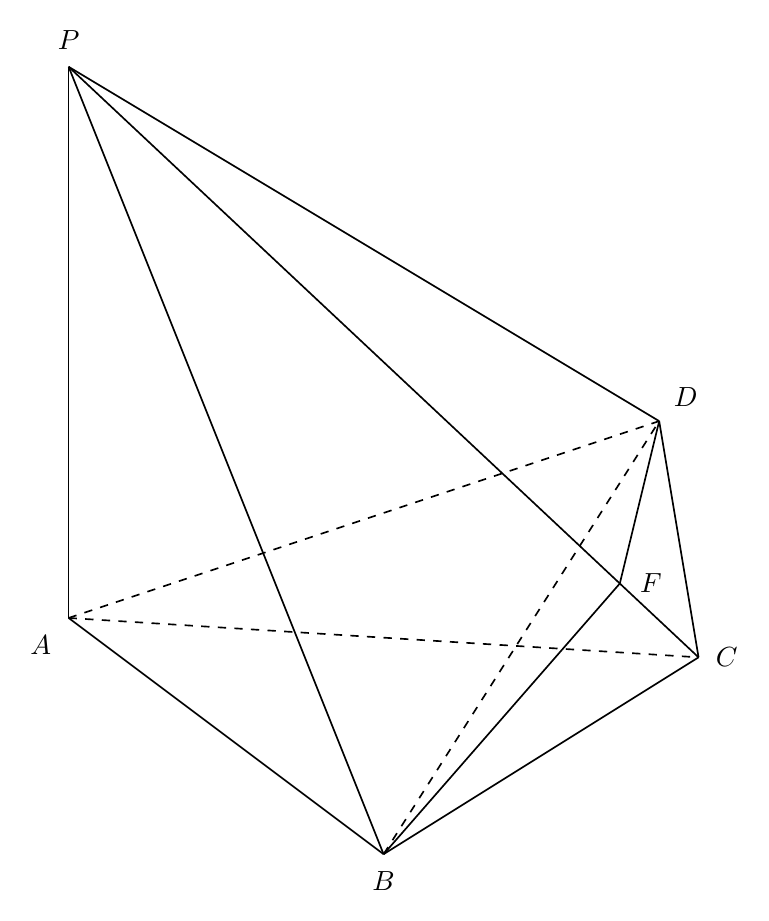
\begin{tikzpicture}[line width=0.6pt, font=\normalsize, inner sep=1pt]
\coordinate (P) at (0,10);
\coordinate (A) at (0,3);
\coordinate (B) at (4,0);
\coordinate (C) at (8,2.5);
\coordinate (D) at (7.5,5.5);
\coordinate (F) at (7.0000000000,3.4375000000);
% solid lateral edges
\draw (P) -- (A);
\draw (P) -- (B);
\draw (P) -- (D);
\draw (P) -- (C);
% solid base edges
\draw (A) -- (B);
\draw (B) -- (C);
\draw (C) -- (D);
% solid segments to F on PC
\draw (B) -- (F);

% hidden base diagonals
\draw[dashed] (A) -- (D);
\draw[dashed] (A) -- (C);
\draw[dashed] (B) -- (D);
% labels placed clear of strokes
\node[above=5pt] at (P) {$P$};
\node[below left=5pt] at (A) {$A$};
\node[below=5pt] at (B) {$B$};
\node[right=5pt] at (C) {$C$};
\node[above right=4pt] at (D) {$D$};
\node[right=6pt] at (F) {$F$};
\draw (D)--(F);
\end{tikzpicture}
